%% this is /book/ioos.txt
\section{Deploying \sciwms{} for the U.S. \ioos{} \comt{} Testbed}

The U.S. Integrated Ocean Observing System (\ioos{}) Coastal and Ocean
Modeling Testbed (\comt{}) was formed to unify otherwise disparate
entities in government, academia and industry to leverage the
proliferation of oceanagraphic data and modeling techniques to combat
natural and man-made coastal stressors by accelerating the turnaround
from research and development to operational application of
society-critical applications including: forecasting, model
comparison, model skill assessment, and algorithmic/parameterization
improvements~\cite{luettich13}.
  
While \sciwms{} is a general software solution for geospatial
visualization, it is a key component in realizing the U.S. \ioos{}
\comt{} mission, facilitating qualitative model comparisons and
aggregation through a unified visualization framework. A crucial
component for the success of the U.S. \ioos{} \comt{} mission is a web
accessable tool for quickly visualizing and assessing a diverse set of
coastal modeling data. \sciwms{} is a general \ogc{} \wms{} solution
for serving rasterized visualizations of geospatial data which has
been deployed for the \comt{} project to provide visualizations of a
wide range of scientific data.

\begin{figure}[ht!]
  \centering
  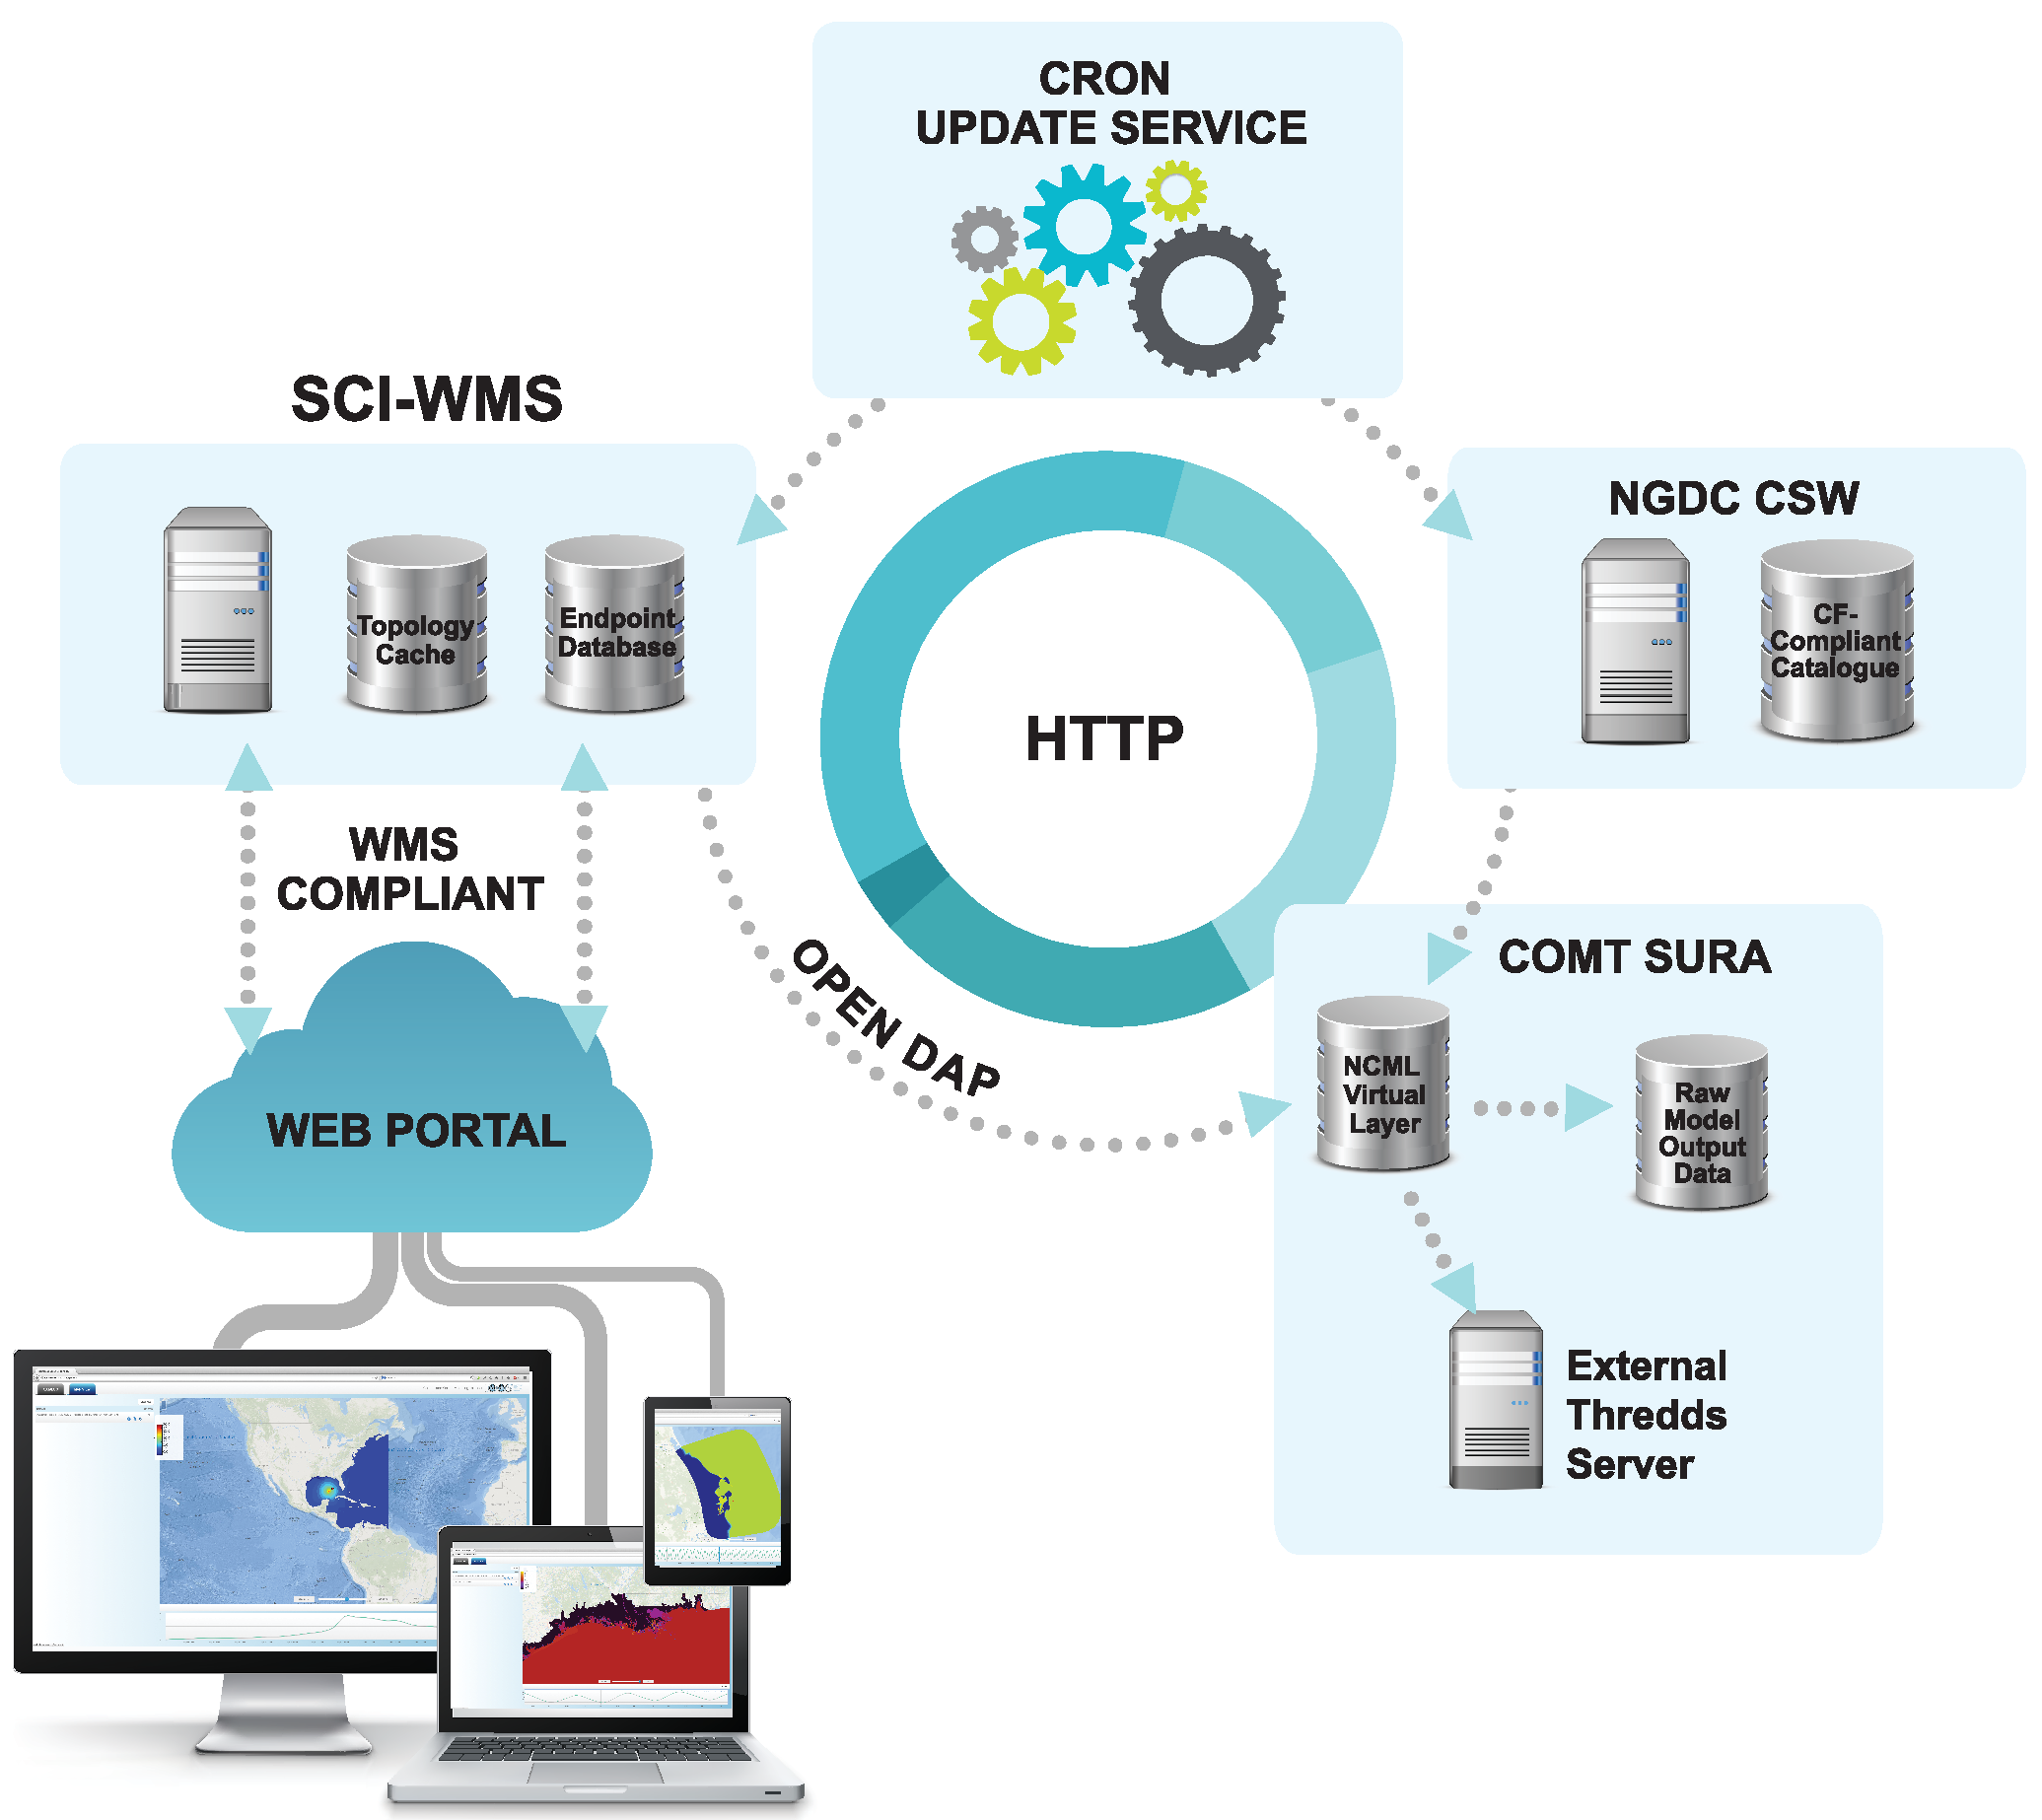
\includegraphics[width=0.7\columnwidth]{../figs/sciwms_overview_v2.pdf}
  \caption{Overview of the \sciwms{} deployment for the U.S. \ioos{}
    \comt{} project. \Sciwms{} updates its topology and endpoint
    database via a nightly service which queries CF-Compliant datasets
    cataloged by \ngdc{}. Model data is hosted on an external web server
    exposed by an \ncml{} facade as a single \netcdf{} data structure
    accessable to \sciwms{} via \opendap{}. \Sciwms{} responds to http
    clients interfacing through a custom built web portal.}
  \label{fig:overview1}
\end{figure}

Figure~\ref{fig:overview1} outlines the cyberinfrastructre behind the
deployment of \sciwms{} for the \comt{} project. The National Oceanic
and Atmospheric Administration (\noaa{}) - National Geophysical Data
Center (\ngdc{}) geoportal indexes public geophysical datasets and
provides an \ogc{} \csw{} service to query datasets by their metadata
attributes. \sciwms{} queries the \ngdc{} Geoportal at regular
intervals updating both the topologies and
\opendap{}~\cite{Cornillon03} links for all new or modified datasets.
Raw coastal data is hosted by the Southeastern Universities Research
Association (\sura{}) on a dedicated server for the \comt{}
project~\cite{luettich12}. Each data set may consist of multiple files
in different formats, and may be the result of very different models
run by various institutions with disparate computing
resources. However, accompanying each dataset is an \ncml{} virtual
layer which exposes each dataset as a single \netcdf{}, \opendap{}
accessable object. Furthermore, the \ncml{} facade presents a
consistent set of meta information in accordance to
CF-Conventions~\cite{cf} providing services like \sciwms{} access to
the raw data through a uniform interface.

Currently, \Sciwms{} is used to visualize data from the first phase
groups of \ioos{} \comt{} program: {\em estuarine hypoxia, shelf
  hypoxia and coastal inundation}~\cite{luettich13}. For each modeling
group, \sciwms{} successfully generates visualizations from
\adcirc{}~\cite{adcirc}, \fvcom{}~\cite{chen06}, \selfe{}~\cite{zhang08} and \slosh{} coastal
modeling algorithms and serves as a use-case of how \sciwms{} can be
leveraged as a scalable solution for delivering consistent
visualizations of scientific data to a diverse community.
